\chapter{Developing The Code}
\label{codechapter}

The new codebase is built in C from the bottom up and follows the basic operation of the old codebase while improving on its performance, organization, and functionality. This newly built codebase splits the tasks of the inherited codebase into a number of logical components. These components are grouped as follows:

\singlespacing
\begin{itemize}
  \item{} Smartwatch Core - Manages all other components.
  \item{} Display Manager - Deals with writing to the display.
  \item{} Clock Driver - Controls RTC\footnote{Real time clock.} and system timers.
  \item{} Bluetooth Driver - Controls Bluetooth interface and protocols.
  \item{} Battery Reader - Checks the battery level of the system.
  \item{} Measurement Controller - Handles the glucose measurement sequence.
  \item{} Button Listener - Records user button presses.
\end{itemize}
\doublespacing
The relationships between all files and components in the new codebase are shown in \figref{fig:new_organization}. In this graph of relationships, it is clear to see that each component branches out from the Smartwatch.h header file, representing the center of the Smartwatch Core. Notice also that modified versions of the Bluetooth library files from the inherited codebase remain, with an additional UART.c file created to provide a better interface to the library.

\begin{figure}[htbp]
    \caption[Organization of New Codebase]{
    A graph of the dependencies within the newly created codebase. All components branch out from the Smartwatch.h header file. On the bottom right, a web of dependencies is seen created from the Bluetooth driver code and associated libraries. On the bottom left, a similar web is shown from the display manager code. The other, simpler components branch linearly from the center.
    }
    \begin{center}
    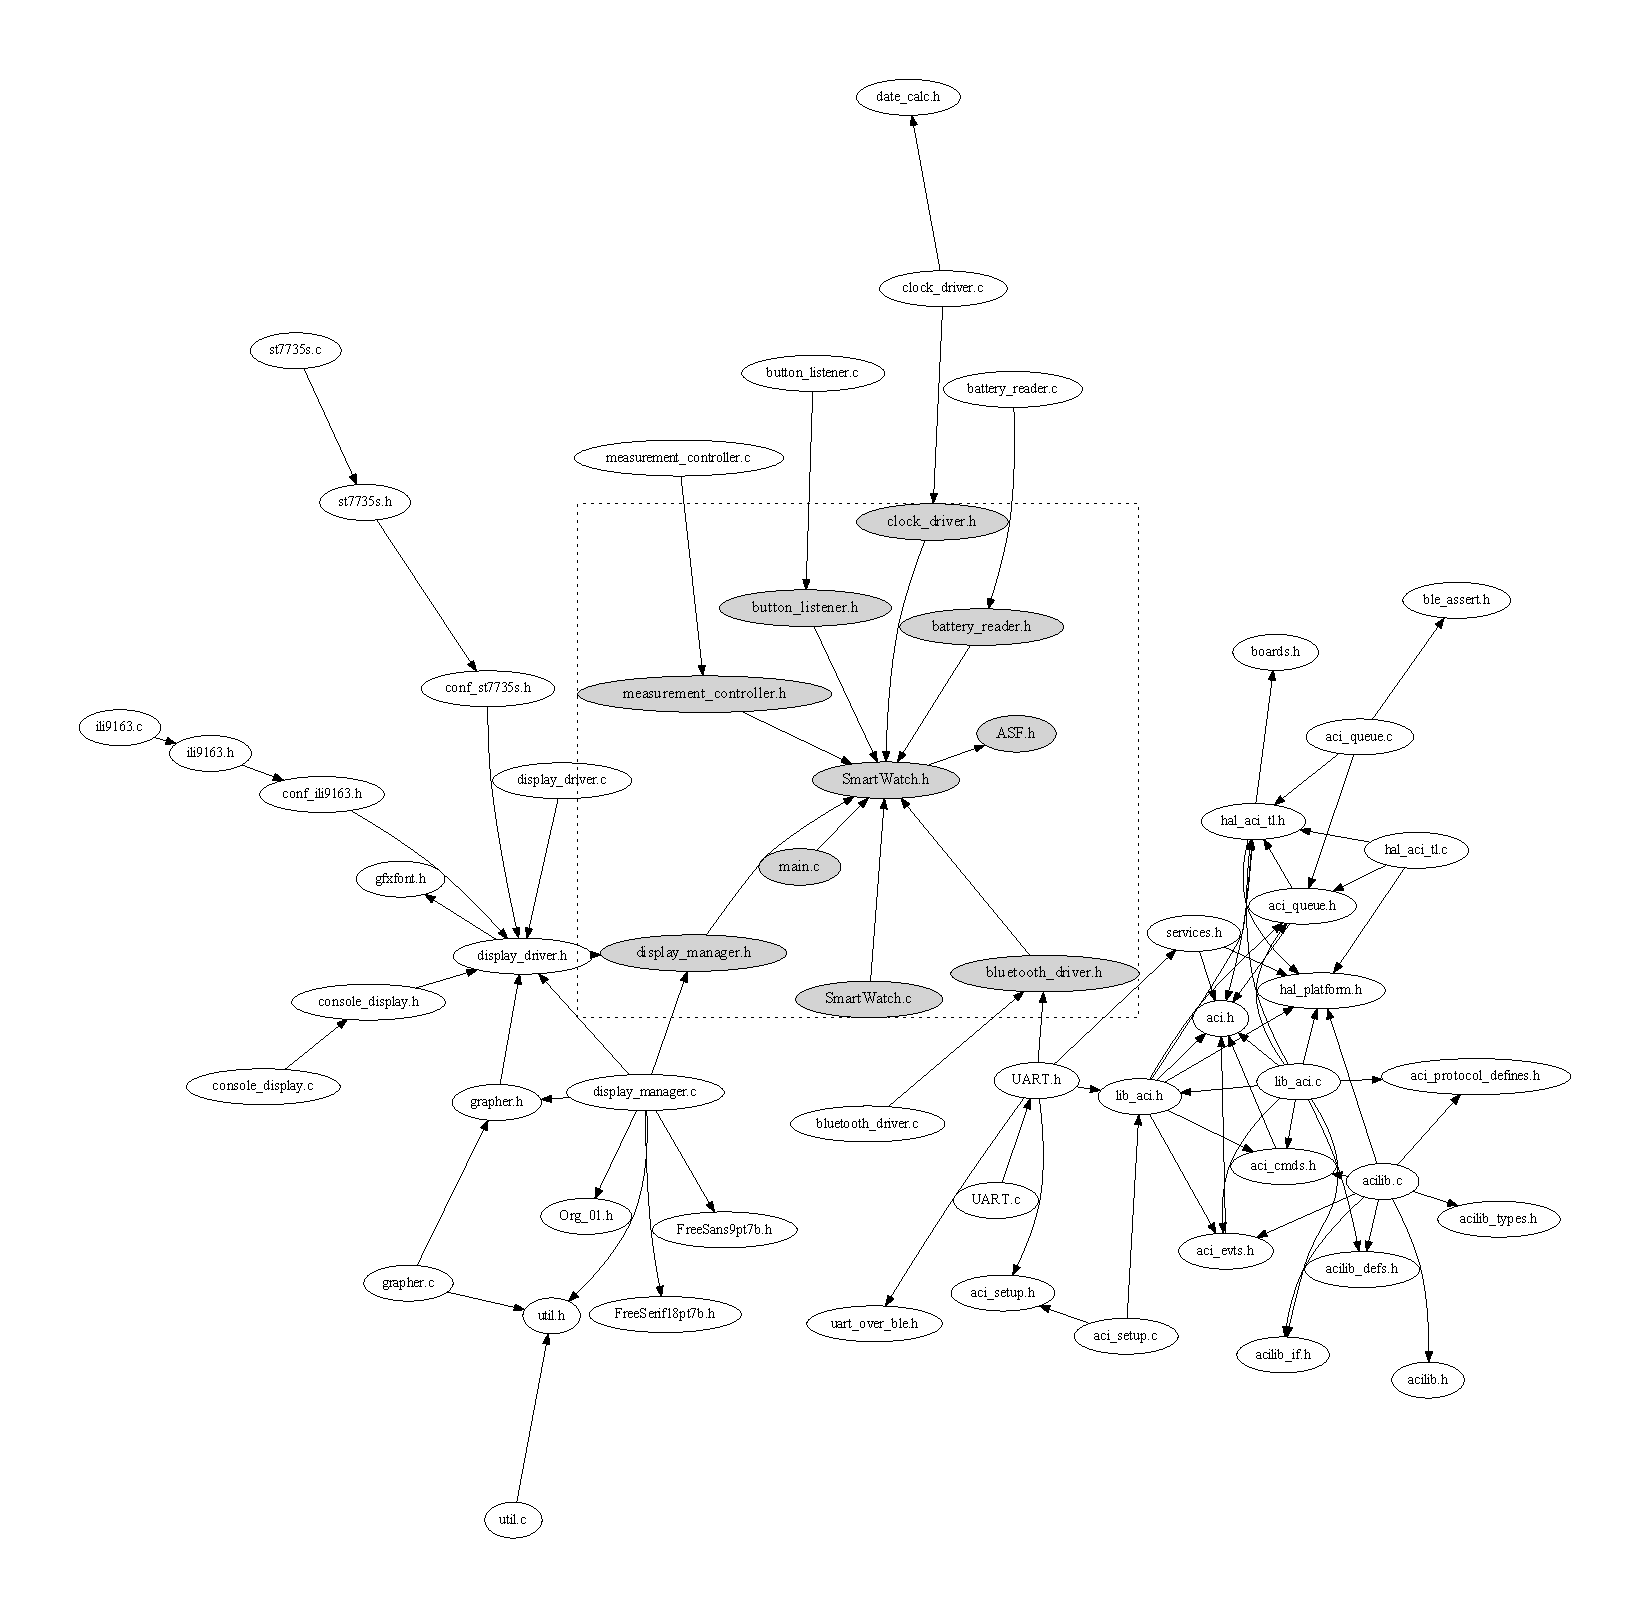
\includegraphics[width=\textwidth,keepaspectratio]{figs/new_organization.pdf}
    \end{center}
\label{fig:new_organization}
\end{figure}


\section{Smartwatch Core}

The smartwatch core is responsible for bringing together all other components of the smartwatch. This core is contained in these files: main.c, Smartwatch.h, and Smartwatch.c. The main function of the newly developed firmware, shown in \ref{main}, follows these logical steps:

\singlespacing
\begin{enumerate}
  \item{} Initialize the system.
  \item{} Check if the smartwatch is active:
\begin{enumerate}
  \item{} If it is active:
\begin{enumerate}
  \item{} Run the smartwatch tasks.
\end{enumerate}
  \item{} If it is not active:
\begin{enumerate}
  \item{} Enter deep sleep mode.
  \item{} Wake up from deep sleep mode on system interrupt.
\end{enumerate}
\end{enumerate}
  \item{} Repeat from number 2.
\end{enumerate}
\doublespacing
When checking whether the smartwatch is active or not, the core checks that a measurement sequence is not in progress, that a Bluetooth message is not being transmitted or received, that the battery level is not currently being read, and that a button input was not received recently. When all these conditions are met, the system is determined to be inactive and deep sleep is entered to conserve battery. Deep sleep will not be exited until a button interrupt or RTC alarm interrupt is detected. A button interrupt indicates that a user wants to view data on the screen, so the display will be woken up as well. On the other hand, when an RTC alarm interrupt occurs a new measurement will be taken by the device, but the display will not be woken up. If any of the conditions for deep sleep are not met then the system must still be active and the associated smartwatch tasks are performed.

The smartwatch task sequence code, as shown in \ref{smartwatch_task}, always calls the Bluetooth and measurement tasks, but will only call the battery and display tasks when the display is activated. The display will be activated when there has been a recent button press and will be deactivated after a preset time, as long as no button presses are read during that time. The battery task only needs called when the display is activated because the battery level is only used for updating the battery level indicator on the screen. A future improvement could be to use the battery level to enter deep sleep mode and prevent wake-up while the battery is at a critical level. Such an improvement would require that the battery task be called at every iteration of the smartwatch task, slightly increasing power usage as the ADC\footnote{Analog to digital converter.} used by the battery reader would need activated more often.

\nl

\section{Display Manager}
The display manager is responsible for writing to the display and managing the state of the smartwatch visual interface. It is a larger library consisting of a display driver that provides an API\footnote{Application programming interface.} for writing to a given display, a grapher that manages an auto-scaling bar graph of the incoming data, and an edited version of the GFX font library\cite{gfxfont} that makes it easier to draw text on the screen. The display manager also relies an a utility file package, consisting of the files util.h and util.c, that implements useful functions for converting numbers into strings\footnote{The functions ftoa\cite{ftoa} and itoa\cite{itoa}.}.

\subsection{Display Task}
The central files of the display manager are: display\_manager.h and display\_manager.c. The display manager task function, which is called in the main smartwatch task and is shown in \ref{display_ui_task}, begins by drawing the header. The header is composed of the current time, battery level, Bluetooth connection status, and date. These portions of the header are designed to be reorderable. This is accomplished by having each header section write to the screen\footnote{I have been using `display' to reference the entirety of the display hardware and `screen' to reference the graphics of the display.} from the left of a given offset position, then return a new offset from which the next header section should begin drawing. After the header is drawn, the window associated with the current state is drawn.

The display manager uses a basic state machine for keeping the state of the current smartwatch window, as shown in \figref{fig:window_state_machine}. At the bottom of each window, text is drawn at either side of the screen that describes the action that would be performed when a user presses the button at the associated side of the smartwatch. The three windows that are implemented are a main window, a notification window, and a graph window. The main window displays the most recent glucose reading and a message about whether there are any notifications. The notification window displays the most recent notifications received by the Bluetooth driver, if there are any. The graph window displays a bar graph representing the most recent measurement data.

\begin{figure}[htbp]
    \caption[Display Window State Machine]{
    A state diagram showing the actions performed by user button presses in each of the viewing windows. At the bottom of each window is text at either side of the screen indicating the action to be performed by the button on the associated side. The images of the display look dithered and faded, due to the quality of the camera and reflections on the screen while the physical display was pictured. The data used to generate the content of the pictured display are simulated.
    }
    \begin{center}
    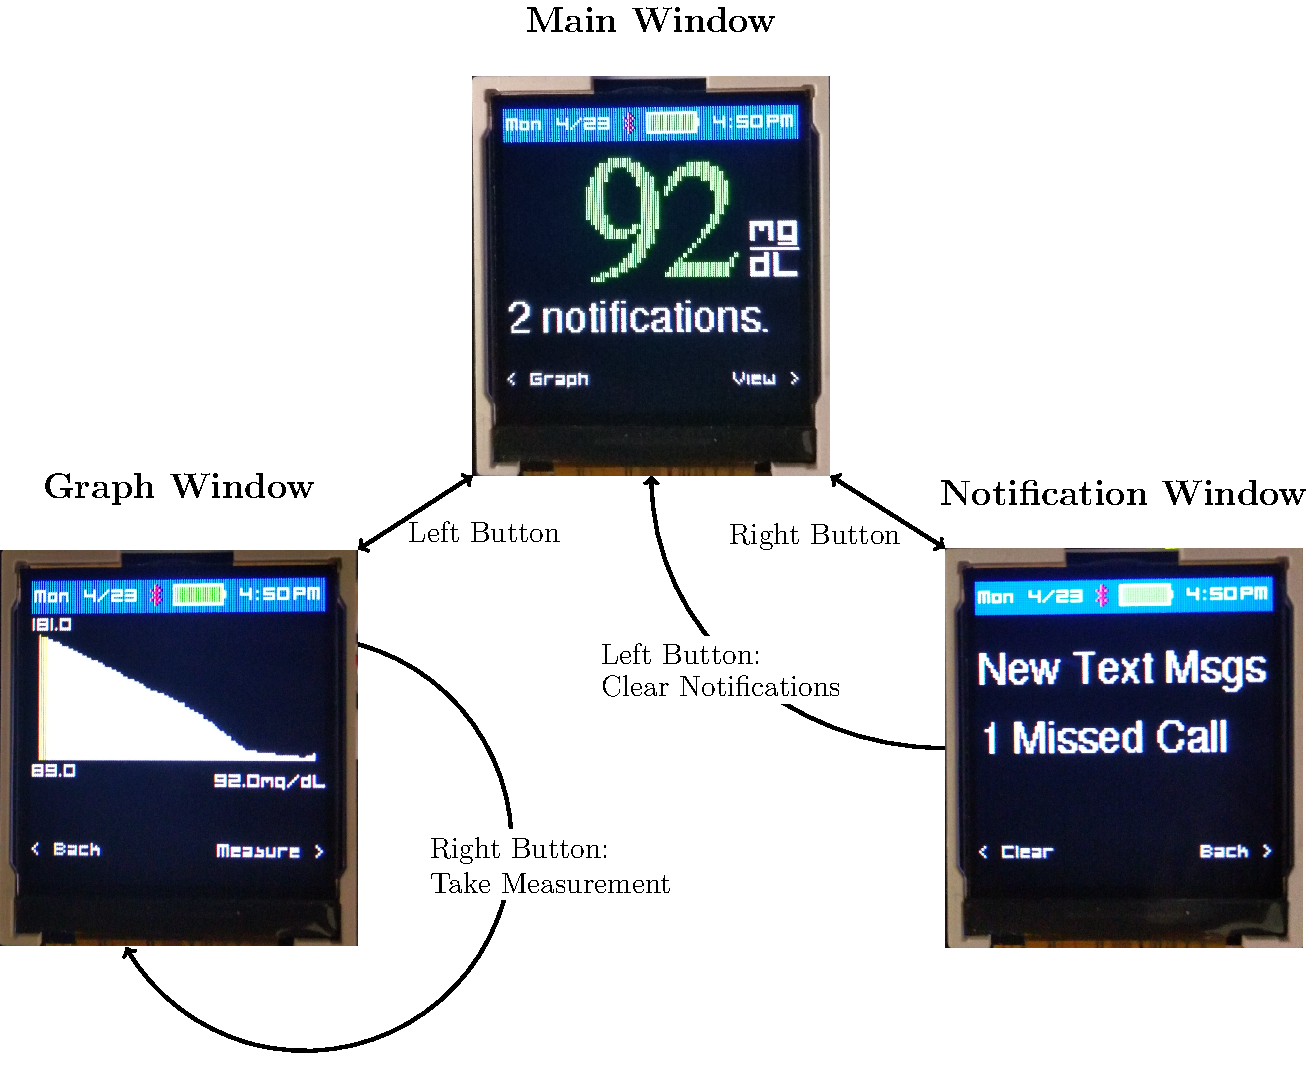
\includegraphics[width=\textwidth,keepaspectratio]{figs/display_window_state_diagram.pdf}
    \end{center}
\label{fig:window_state_machine}
\end{figure}

\subsection{Grapher}
The files that make up the grapher, which manages the bar graph displayed in the graph window, are: grapher.h and grapher.c. The grapher keeps a set of data points and an associated set of precomputed bar heights in two circular buffers\footnote{A circular buffer is an array that, when overfilled, will begin overwriting itself from its beginning.\cite{wikiCB}}. When a new data point is received by the grapher, the grapher will determine if the minimum or maximum values of the graph have changed and then precompute the bar heights for the data points that need updated. The formula for computing the bar height of a given data point is given in the following equation.
% \equref{eq:bar_height}:

\begin{equation} % \label{eq:bar_height}
\text{bar\_height} = \frac{\text{data\_point}-\text{data\_point}_\text{min}}{\text{data\_point}_\text{max}-\text{data\_point}_\text{min}}(\text{bar\_height}_\text{max}-\text{bar\_height}_\text{min}) + \text{bar\_height}_\text{min}
\end{equation}
\nl
\indent The grapher provides two functions for drawing the graph. The first function assumes that it must clear the area of the screen itself and so is unused by the firmware, as writing to every pixel within the bounds of the graph will slow down the display writing process. This first, na\"ive function is shown in \ref{graph}. In order to speed up the writing process, a second function is provided, which is shown in \ref{graph_smart_sizing}. The second function assumes that pixels do not need to be cleared by the grapher, rather it is the responsibility of the caller to clear the screen before the graph is drawn. This function provides a hint to the caller about where in the screen the graph was drawn by returning a bounding box of the drawn graph. Every pixel within the bounds of the graph would still need drawn for a full set of data, as the bounding box returned from the function will be the same as the bounds of the drawable graph area; however, the total performance improvement seen by allowing the caller to manage the erasure of the graph is still enough to make this second function better than the first.

\subsection{Display Driver}
The display driver provides an API for writing graphics to a given display. Its main files are: display\_driver.h and display\_driver.c. The display driver provides simple functions that draw pixels, lines, rectangles, and text in up to 4096 different colors to the screen. A buffering strategy is used to improve speed, meaning that when graphics data is to be written to the display, it is first placed in a buffer whose size is equal to the dimensions of the target screen. When the graphics data is ready to be written, this buffer is then copied to the target screen. This buffering strategy provides visually smoother drawing than if each pixel was individually drawn to the screen. Individually drawing each pixel to the screen would create a slight delay between the calculation and drawing of each pixel. By using a buffer, the pixels to be drawn can be calculated beforehand and no visual delay would be seen resulting from these calculations.

A problem with the buffering strategy is that a large region of memory is needed for storing the buffer. For instance, if a single pixel is represented using 18-bits and the dimensions of the screen were 200$\times$200 pixels, then $200\times200\times18 = 720000$-bits would be needed to store all the information. Additionally, since data is usually stored in multiples of 8-bits, a na\"ive structure for storing this example data could use $200\times200\times32 = 1280000$-bits -- which is about 156KB. Since the MCU only has 32KB total SRAM\footnote{Static random-access memory.}, such a structure would be impossible to store in SRAM alone. One solution for reducing the size of the buffer is to store only a couple bits to represent a pixel. If it is known that 4 colors are used by a display, then one can simply store each pixel as a number within 0 to 3 -- that is, as a 2-bit number. When it is time to draw the pixel, it can be converted to the necessary number of bits before being written to the display. Continuing with the example above, the resulting storage would need at least $200\times200\times2 = 80000$-bits, about 10KB of data. Another solution may be to store the buffer in flash memory, of which the MCU provides 256KB, or to use external memory. All of these solutions share the disadvantage that they would result in a slightly slower display writing process. Due to this disadvantage and the fact that the screen used by the smartwatch is sufficiently small, none of these solutions are used by the display driver. These solutions are left as possible future improvements however, should future modifications of the smartwatch judge them necessary.

The solution used by the display driver for reducing the size of the buffer is to use the minimum pixel resolution of the target display and to store data in the buffer contiguously. With a 128$\times$128-pixel target display screen at a minimum resolution of 12-bits per pixel, the resulting buffer would be $128\times128\times12 = 196608$-bits, or 24KB. Due to the relatively small size of the rest of the codebase, this large block of memory is able to fit into SRAM and no other solution is needed. Still, remember that data is usually stored in multiples of 8-bits, so the problem of storing each of these 12-bits remains. To store the pixel data, the display driver splits two pixels across three groups of 8-bits. The resulting structure\footnote{An alternative structure could be created using the C language concept of bit fields\cite{wikiBF}.} is an array of 8-bit elements with $\frac{3}{2}\times128\times128$ elements, where a simple mapping of pixel positions to array positions is used for determining where a pixel is to be written into the array. This mapping is given in the following equations:

\begin{eqnarray}
\text{array\_position} &=& \text{array\_x} + (\frac{3}{2}\times \text{pixel\_y} \times \text{display\_width})
\\
\text{array\_x} &=& \left\{\mat[\frac{3}{2}\times \text{pixel\_x} &;&\text{pixel\_x is even}\\\frac{3}{2}(\text{pixel\_x}-1)+1 &;&\text{pixel\_x is odd}]\right.
\end{eqnarray}
\nl
\indent In addition to a buffering strategy, the display driver uses partial screen rendering to increase speed. This means that as the display driver draws pixels, it keeps track of the furthest pixels it has drawn. Using a bounding box containing these pixels, the display driver can update the screen with only the pixels within the box. This significantly increases the speed of the display write process when the updated pixels are localized to certain portions of the screen, as time will not be spent on drawing pixels that were not updated. The code that achieves writes to the buffer and updates the bounds for partial screen rendering is shown in \ref{disp_write_pixel_at}.

The display driver also uses a concept called graphics grouping\footnote{This concept is named so by me.}, which complements the partial screen rendering strategy and helps simplify the process for removing and updating graphics. Graphics grouping simply stores the bounding box of graphics to be drawn, so that the driver knows what region needs updating when the graphics update or need removed. In the display driver, each graphics group is given a unique ID. When a graphics group is written to in the display driver, the previous graphics group with the same ID provides a bounding box that is then cleared in the buffer. After the old bounding box has been cleared, a new bounding box is stored for the new graphics that were just written. The result is that the display driver will automatically clear the old data of a graphics group whenever that graphics group is written to. Since the display driver uses a buffering strategy, any delays imposed by this grouping process of removing and writing to the same area of the buffer will not result in visual delays on the screen. The code for writing a string to a graphics group is shown in \ref{disp_write_str_group}.

The display manager uses the graphics grouping capabilities of the display driver extensively, and optimizes the process further by committing the buffer to the physical display following the drawing of most groups. Additionally, the display manager will only call the display driver to draw to the screen when the content of the screen will be updated, opposed to on every main loop iteration. This saves further time as the display driver will only need to overwrite its buffer in cases where the data of the buffer will actually change. Example usage of graphics grouping by the display manager is given in the main window drawing command, shown in \ref{updateMainDisplay}.

Finally, as mentioned, the display driver provides an API for writing to any given display. Implementations for two LCD\footnote{Liquid crystal display.} controllers are written, as well as an implementation for the standard output stream, which is used to aid debugging. These LCD controllers are the ST7735S\cite{ST7735S} and ILI9163\cite{ILI9163}, which are supported for use with 12-bit color resolution only. The controllers are written for an SPI\footnote{Serial peripheral interface.} connection, but implementations for parallel connections can be written without changing the display driver code. Support for more color resolutions and larger screen dimensions are left as future improvements that can be made to the display driver.

\nl

\section{Clock Driver}
The clock driver is responsible for managing the current time and the various system timers. It is contained in these files: clock\_driver.h, clock\_driver.c, and date\_calc.h. The target MCU provides five 16-bit timers, three 24-bit timers, and a 32-bit RTC. A set of two 16-bit timers can be cascaded by the hardware into a 32-bit timer. The RTC is configured to run at 32.768KHz, in order to generate a precise one second period. The other timers that are used by the smartwatch are configured to run at 8MHz, the same as the program clock speed of the MCU. Higher frequencies can be configured, but are not used as they do not provide enough performance improvement to offset their extra power requirements. The only hardware component where the extra performance of a higher frequency clock should be used is in the display SPI, which runs at 48MHz. The display SPI is configured to use a higher clock frequency than the rest of the smartwatch in order to speed up the display writing process.

\subsection{Real Time Clock}
The clock driver uses the RTC to keep the current time. The default time and date are automatically set to the current time and date during compiling, but can be reset using a Bluetooth command should the time or date need correcting. An RTC alarm interrupt is configured as well, which will wake up the smartwatch if needed and then trigger a new glucose measurement. After each RTC alarm interrupt, a new alarm is configured for the next scheduled reading. This periodic measurement can be disabled, by setting the alarm period to zero. The alarm code for the RTC is shown in \ref{rtc_alarm_callback}.

The clock driver relies on the date\_calc.h utility file to accurately follow the Gregorian calendar. This utility file operates on Gregorian dates using algorithms described by Gary Katch\cite{datecalc}. Whenever the current time updates and a new day begins, the next date is calculated using these algorithms and the current date is updated. Additionally, each time the current second changes, the display manager will blink the time delimiter\footnote{The colon between the hour and minute of a written time, i.e. in 12:34.} of the displayed time, similarly to most other digital clocks.

\subsection{Timers}
The clock driver manages four timers to be used by the smartwatch. These timers are a screen timer, pulse timer, battery timer, and button timer. The button timer is configured to trigger an interrupt every millisecond, while the other timers trigger separate interrupts each second. When an interrupt is triggered for a timer, an associated counter is decremented. When that counter reaches zero, the timer is disabled and a timeout flag is raised for that timer. The clock driver provides functions for resetting the timeout of each timer, which will set the counter appropriately and re-enable the timer. Each timer follows the same basic code structure. The code used for running the screen timer is shown in \ref{screen_timer_callback}.

The screen timer is reset by the smartwatch core each time the display is activated, either by a button interrupt or software request. While the counter for this timer has not reached zero, the display will be determined as active and will be powered. When the counter reaches zero, the smartwatch core will deactivate the display and place it into sleep mode.

The pulse timer is used by the measurement controller while it is taking a measurement. It is used for allowing the implant time to power up and settle on a value, as well as for taking multiple data points over a period of time in order to find an average measurement.

The battery timer is used by the smartwatch core to periodically read the battery level through the battery reader. Additionally, the smartwatch core will set the battery counter to zero in order to trigger the battery reader each time the display is reactivated, so that the displayed battery level always starts at the most recent value.

The button timer is used by the button listener for debouncing the smartwatch buttons. It is the only timer that counts in milliseconds, which allows the buttons to be debounced at a speed that does not conflict with additional button presses from a user.

\nl

\section{Bluetooth Driver}
The Bluetooth driver is responsible for handling messages received over Bluetooth and interacting with the ACI\footnote{Application controller interface.} BLE\footnote{Bluetooth low energy.} library. The core files of the Bluetooth driver are: bluetooth\_driver.h and bluetooth\_driver.c. These files parse received Bluetooth messages and perform certain actions based on each message. Additionally, when a device is connected to the smartwatch through Bluetooth, the Bluetooth driver will send to that device a message containing the most recent glucose measurement.

\subsection{Messaging Protocol}
A message received by the Bluetooth driver from a connected device, such as a smartphone running the corresponding app, will trigger an action when the message begins with a certain letter. The subsequent characters of the message are then used as parameters for that action. While it is easy to add additional commands and actions, should they be needed in future editions of the smartwatch, the currently supported actions are as follows:

\singlespacing
\begin{itemize}
  \item{} `1': Sets the 1st notification to the subsequent text.
  \item{} `2': Sets the 2nd notification to the subsequent text.
  \item{} `R': Sets the period for the periodic measurement to the subsequent number of seconds.
  \item{} `D': Sets the date and time to the subsequent text, formatted: yyyy mm dd hh mm ss. \footnote{Year, month, day, hour, minute, then second.}
\end{itemize}
\doublespacing
Notice that it is the responsibility of the connected Bluetooth device to construct notifications to be displayed on the smartwatch. The Bluetooth driver will simply set the associated notification in the smartwatch to the received text, up to a length limit. On receipt of a notification, the Bluetooth driver will also set a flag to indicate that there are notifications to be displayed. The display manager uses this information while displaying the number and content of notifications.

The Bluetooth driver keeps a circular buffer of received messages, and will parse each message in the order received. Should a large number of messages be received in a short time, the Bluetooth driver will overwrite the oldest message in the buffer. A future improvement could be to add a field for priority in the message format, which would be used to determine the order for replacing overcrowding messages.

No special command sequence is used when sending data from the smartwatch over Bluetooth, as the smartwatch supports only one type of outgoing command. The Bluetooth driver simply transmits the glucose data found on each new measurement reading. It is the responsibility of the connected device to interpret the data sent to it as a glucose measurement. Should a Bluetooth device not be connected, the Bluetooth driver will wait until a new connection is made before sending the most recent glucose data. The Bluetooth task code is shown in \ref{bt_task}.

\subsection{ACI BLE Library}
The smartwatch uses the nRF8001\cite{NRF8001} to manage its BLE connection and the Bluetooth driver uses the ACI BLE library to interact with it. The ACI BLE library is modified for use with the target MCU from Adafruit's nRF8001 Arduino drivers\cite{libaci}. The core interface to the ACI BLE Library consists of these files: UART.h and UART.c. Using the ACI BLE library, the Bluetooth driver waits for the nRF8001 to indicate that an event has occurred, then connects to the nRF8001 over SPI to receive the event. Once the event and associated parameters have been received, the event is handled based on its type. The supported event types are as follows:

\singlespacing
\begin{itemize}
  \item{} Device Started Event: Sent every time the device starts.
  \item{} Echo Event: Mirrors the last echo command.
  \item{} HW Error Event: Sent when a hardware error occurs.
  \item{} Response Event: Generic response to a command.
  \item{} Connected Event: Link connected.
  \item{} Disconnected Event: Link disconnected.
  \item{} Bond Status Event: Result of completed pairing.
  \item{} Pipe Status Event: Pipe bitmap for available pipes.
  \item{} Timing Event: Sent when the radio state changes.
  \item{} Data Credit Event: Sent when transmit credits are available.
  \item{} Data ACK Event: Acknowledgement to previous command.
  \item{} Data Received Event: Sent when new data is available..
  \item{} Pipe Error Event: Sent on software error.
  \item{} Display Passkey Event: To communicate passwords.
  \item{} Security Key Request Event: Sent on password request.
\end{itemize}

\doublespacing
When the nRF8001 is first started, the ACI BLE library attempts to configure it. The nRF8001 is configured using precompiled setup configuration data, which sets device information such as the connection name, timeout limits, and security details. Once the nRF8001 is setup, the ACI BLE library will trigger an attempt to bond with a device. Until a device is connected, the nRF8001 will continuously retrigger a bonding sequence after each timeout. When a device is connected, the Bluetooth driver is notified and sets an appropriate flag. This flag is used by the display manager to render the Bluetooth connection indicator. When a connected device is disconnected or a hardware error occurs, the connection flag is reset and the ACI BLE library triggers another attempt to bond with a device. The nRF8001 acts as a slave device, meaning that it is the responsibility of a Bluetooth enabled device to initiate pairing with the smartwatch. Similarly, it is the responsibility of a connected device to reconnect with the smartwatch should the connection be lost.

While a Bluetooth device is connected to the smartwatch, data can be transmitted to or from the paired device. When data is received, the ACI BLE library will send the received data to the message buffer in the Bluetooth driver and then trigger a callback in the Bluetooth driver. This callback simply records that a new message was received and increments the next position of the received data buffer. After data is successfully sent from the smartwatch over Bluetooth, the ACI BLE library will trigger a similar callback in the Bluetooth driver to signal that the transmission has completed.

\nl

\section{Battery Reader}
The battery reader is responsible for reading the current battery level and is built from these files: battery\_reader.h and battery\_reader.c. The battery reader uses the ADC of the MCU to measure battery voltage. Voltage taken directly from the battery -- which has a maximum voltage of about 4V -- is divided by two using a voltage divider circuit, then is fed into the MCU for use as the ADC input. This input is compared to the converted voltage level powering the MCU, which is 3.3V. The battery reading process works because the actual voltage of the battery is higher than the voltage powering the MCU. This means that the difference between the battery voltage and MCU voltage can be measured in order to estimate the battery level of the smartwatch. When the battery has a full voltage, the battery level is read as maxed. When the battery voltage is close to the voltage powering the MCU, the battery level is read as nearly empty. The actual voltage of the battery is divided by two before it is fed to the ADC, meaning that the calculation for the battery level uses 2V as the maximum battery level and 1.65V as the minimum battery level. The battery level is calculated as a percentage of a maximum value, given to the battery reader from the display manager in order to make it easier to draw the battery level indicator. The code that calculates the battery level is shown in \ref{battery_task}.

\nl

\section{Measurement Controller}
The measurement controller is responsible for taking glucose measurements and is built from these files: measurement\_controller.h and measurement\_controller.c. The measurement controller stores the most recent glucose value, while previously-measured glucose information is stored in the display manager by the grapher. Additionally, glucose information will be sent over Bluetooth to any connected device, which may store further copies of the glucose information. It is assumed that in order to store the glucose information of real users, the distributors of a glucose-monitoring smartwatch supplied with this firmware have made sufficient steps to follow HIPAA\footnote{Health Insurance Portability and Accountability Act of 1996.\cite{HIPAA}} and any other related regulations or laws. This assumption is made also for regulations or laws in countries other than the United States of America, should they apply. It is important to note that this firmware, on its own and in its current state, may not be satisfactory for commercial use without additional security features, such as the encrypting of stored information. Encryption of data and other modifications necessary to produce a commercial edition of this firmware are left as future improvements.

It is important to note that in order to take measurements, the measurement controller only requires that a signal of a certain frequency be given to it. Due to this, the smartwatch can be repurposed for functions other than measuring glucose, so long as the desired data is encoded as a frequency signal.

\subsection{Glucose-Measuring Implant}
The smartwatch is designed to interface with an implantable, glucose-measuring device developed by the sponsor company. This implant sits under the skin and is powered by a solar cell. The implant receives power from an array of LEDs\footnote{Light emitting diodes.} that sit at the bottom of the smartwatch. When powered, the implant generates an electric current based on the amount of glucose it detects in its surroundings. The implant will then blink an LED at an appropriate frequency based on the glucose amount. The smartwatch uses an array of photodiodes to detect the transmitted light signal and determine its frequency. A filter sits between the photodiodes and LEDs on the smartwatch in order to filter out all incoming light except the light generated from the implant. The signal frequency measured by the measurement controller is then converted into a glucose value.

\subsection{Measurement Sequence}
The measurement controller begins a measurement sequence by turning on the LED array for a number of seconds, which allows the implant to power on and settle at a glucose value. The measurement controller then triggers a frequency capture event using an external interrupt on the photodiode array pin. This frequency capture event is used to determine the frequency of the received signal. A large number of frequency samples are taken, and the average of these values is recorded. This process is repeated each second for a number of seconds, then the recorded values are averaged into a final frequency value. The final frequency value is then converted into a glucose value using a conversion algorithm. The measurement task code that accomplishes this is shown in \ref{measurement_task}.

\nl

\section{Button Listener}
The button listener is responsible for recording button interrupt events and is built from these files: button\_listener.h and button\_listener.c. The button listener simply initializes an external interrupt for each of the two smartwatch buttons, then will set a flag for the associated button whenever its interrupt occurs. The smartwatch core periodically polls the button listener for recent button presses. On receipt of a button read from the smartwatch core, the button listener will clear its button flags and continue waiting for additional button presses.

The button listener configures its external interrupts to be enabled during deep sleep mode, in order to allow the device to be woken up when a user presses a button. In cases where a button press wakes up the device, the button flags will be cleared, so as to not trigger any action usually tied to the buttons while the device is awake.

A timer is used for debouncing the buttons. When a new external interrupt occurs after a button press, a timer will begin counting down from a preset number of milliseconds. Any additional external interrupts that occur before the timer reaches zero are discarded. This prevents a single button press from being read as multiple presses due to the physical behavior of the button. Other implementations for button debouncing are possible, including hardware solutions\cite{debounce}. These solutions were not used as the timer method for debouncing was found to be adequate during testing. A recommended future improvement to the smartwatch would be the addition of capacitors on the button inputs for a hardware solution to debouncing. Sample code from the button listener is shown in \ref{is_button_interrupt}.
